\documentclass[catalan, a4paper, nobib]{tufte-handout}

% encoding
\usepackage[utf8]{inputenc}
\usepackage[T1]{fontenc}
\usepackage{lmodern}
\usepackage{babel}

% formatting and fixes
\frenchspacing
\usepackage[style=spanish]{csquotes}
\MakeAutoQuote{«}{»}

% general design preferences (page, newthought indent/space, margins,  ass options, ...)
%%\setlength{\parskip}{10pt}
%%\pagestyle{plain}

% ADD ANY SPECIFIC PACKAGES HERE
% (CHEMISTRY, CODE, PUBLISHING)
\usepackage{booktabs}
\usepackage{circuitikz}
\usepackage{siunitx}
\usepackage{amsmath}
\usepackage{minted}

% other options

\graphicspath{
    {tests/}
}

% hyperlink setup / metadata
\usepackage{hyperref}
\AfterPreamble{\hypersetup{
  %%pdfauthor={},
  %%pdftitle={},
  %%pdfsubject={},
}}

% document metadata
\author{54894677W}
\title{Treball final CSL}
\date{5-5-2023}

\begin{document}

\maketitle

\section{Estudi de les ressonàncies del cristall de quars}

\newthought{Pas 1:} El conjunt sèrie $R_m$ - $L_m$ - $C_m$ té una impedància $Z_m(\omega) = R_m + j(L_m \omega - \frac{1}{C_m \omega})$. Podem observar que la funció $|Z_m|(\omega)$ té un únic mínim relatiu o, d'altra banda, que la part imaginària de $Z_m(\omega)$ es cance\l.la per $\omega = \frac{1}{\sqrt{L_m C_m}}$. Sigui com sigui, s'arriba a la conclusió que el conjunt té una única freqüència de ressonància situada a $f_0 = \frac{1}{2\pi} \frac{1}{\sqrt{L_m C_m}}$.

\newthought{Pas 2:} Evaluem per casos la impedància del conjunt.

\begin{description}
  \item[$f = f_0$:] Com $Z_m = R_m$ el conjunt es pot substituir per un resistor.
  \item[$f < f_0$:] Intuitivament, la impedància d'un condensador a freqüències baixes és més gran que la d'un inductor. Analíticament, si $\Im(Z_m) = L_m \omega - \frac{1}{C_m \omega}$ per una $\omega < \omega_0$, llavors $\frac{1}{C_m \omega} > \frac{1}{C_m \omega_0}$ i $L_m \omega < L_m \omega_0$ resultant en una part imaginària negativa. Podem aleshores substituir el conjunt per un resistor en sèrie amb un condensador. \sidenote{En sèrie la impedància es suma. La impedància d'un condensador és $-j\frac{1}{C \omega}$ (part imaginària negativa). En para\l.lel caldria un inductor.}
  \item[$f > f_0$:] Amb el mateix raonament que abans obtenim que la part imaginària es positiva. Per tant, podem substituir el conjunt per un resistor en sèrie amb un inductor.
\end{description}

\begin{table}
  \begin{center}
    \begin{tabular}{@{}lccc@{}}
      \toprule
      & $f<f_0$ & $f = f_0$ & $f > f_0$ \\
      \midrule
      Circuits equivalents:
      &
      \begin{circuitikz}[transform shape, scale=0.6, baseline]
        \draw (0,0) to[short, o-] ++(0.25,0) to[R=$R_m$] ++(1.5,0) to[C=$C$] ++(1,0) to[short, -o] ++(0.25,0);
      \end{circuitikz}
      &
      \begin{circuitikz}[transform shape, scale=0.6, baseline]
        \draw (0,0) to[short, o-] ++(0.25,0) to[R=$R_m$] ++(1.5,0) to[short, -o] ++(0.25,0);
      \end{circuitikz}
      &
      \begin{circuitikz}[transform shape, scale=0.6, baseline]
        \draw (0,0) to[short, o-] ++(0.25,0) to[R=$R_m$] ++(1.5,0) to[L=$L$] ++(1.25,0) to[short, -o] ++(0.25,0);
      \end{circuitikz}
      \\
      \bottomrule
    \end{tabular}
  \end{center}

  \caption{Comportament elèctric del cristall de quars al voltant de la ressonància sèrie}
\end{table}

\newthought{Pas 3:} El para\l.lel $C_e$ sí provoca la aparició d'una freqüència de ressonància adicional superior a la ressonància sèrie. En aquesta segona ressonància el conjunt té una impedància molt gran.

\newthought{} Per freqüencies més baixes que $f_0$ el conjunt sèrie es pot substituir per un resistor i un condensador de valor indeterminat. Aquest últim conjunt pero, en para\l.lel amb un altre condensador no provoca la aparició de cap frequència de ressonància\sidenote{La part imaginària de la impedància no es pot cance\l.lar per cap $0 < \omega < \infty$.}. En canvi, per freqüencies més altes que $f_0$ es té un bloc sèrie resistor-inductor en para\l.lel amb un condensador. Aquesta última configuració té una freqüència de ressonància per $\frac{1}{\sqrt{L C_e}}$.

\newthought{} El bloc $R - L$ en para\l.lel amb $C$ és més habitual. La resistència $R_m$ és suficientment petita en relació a $L$ com a per a tractarla com la resistència interna d'un inductor no ideal. Aixi doncs podem reescriure el conjunt com a la figura \ref{fig:high_freq_equiv}. On $R_p$ és $R_m Q_b^2$ i $L_p$ és practicament $L$. En freqüència de ressonància aquest conjunt te una impedància real $R_p$. Com $Q_b$ és molt gran aquesta impedància també ho serà.

\begin{marginfigure}
  \begin{center}
    \begin{circuitikz}
      \draw (0,0) to[short, o-] ++(0.5,0) to[short] ++(0,1) to[L=$L_p$]++(2,0) to[short] ++(0,-2);
      \draw (0.5,0) to[C=$C_e$] ++(2,0) to[short, -o] ++(0.5,0);
      \draw (0.5,0) to[short] ++(0,-1) to[R=$R_p$] ++(2,0);
    \end{circuitikz}
  \end{center}
  \caption{Circuit equivalent per excitacions amb freqüència superior a la ressonància sèrie}
  \label{fig:high_freq_equiv}
\end{marginfigure}

\section{Estudi analític de la resposta freqüencial del circuit de mesura}

\newthought{Pas 4:} Apliquem anàlisi per nodes al circuit de la figura \ref{fig:circuit_1} i obtenim la següent equació.

\begin{gather*}
  V_o \left [ \frac{1}{R_o} + \frac{1}{R_m + L_m s + \frac{1}{C_m s}} \right ] = V_{in} \left [ \frac{1}{R_m + L_m s + \frac{1}{C_m s}} \right ]
  \\
  H(s) = \frac{V_o(s)}{V_{in}(s)} = \frac{\frac{1}{R_m + L_m s + \frac{1}{C_m s}}}{\frac{1}{R_o} + \frac{1}{R_m + L_m s + \frac{1}{C_m s}}}
\end{gather*}

\newthought{} Després de normalitzar la funció de xarxa obtenim:

\begin{gather*}
  H(s) = \frac{R_o}{L_m} \cdot \frac{s}{s^2 + \frac{R_m + R_o}{L_m} s + \frac{1}{L_m C_m}}
\end{gather*}

\newthought{} Aquesta funció de xarxa clarament correspon a un filtre passabanda de segon ordre. De segon ordre perquè hi ha dos pols i passabanda perquè hi ha un zero per $s = 0$ i un altre per $s \rightarrow \infty$.

\begin{figure}
  \begin{center}
    \begin{circuitikz}
      \draw (0,0)node[below]{$+$} to[short, o-] ++(0.25,0) to[R=$R_m$] ++(1.5,0) to[L=$L_m$] ++(1.5,0) to[C=$C_m$] ++(1.5,0) to[short, -*] ++(0.25,0) to[short, -o] ++(1.5,0)node[below]{$+$};
      \draw (5,0) to[R=$R_o$] ++(0,-2);
      \draw (0,-2)node[above]{$-$} to[short, o-*] ++(5,0) to[short, -o] ++(1.5,0)node[above]{$-$};
      \draw (-0.5,0) to[open=$v_{in}(t)$] ++(0,-2);
      \draw (6,0) to[open=$v_o(t)$] ++(0,-2);
    \end{circuitikz}
  \end{center}
  \caption{Esquema del circuit de mesura menyspreant $C_e$ i eliminant el conjunt $v_g(t)$ - $R_o$}
  \label{fig:circuit_1}
\end{figure}

\newthought{Pas 5:} Per esbrinar les característiques del filtre fem servir les formules deduides per un filtre passabanda de segon ordre genèric.

\begin{gather*}
  H(s) = \frac{R_o}{L_m} \cdot \frac{s}{s^2 + \frac{R_m + R_o}{L_m} s + \frac{1}{L_m C_m}} = k \cdot \frac{s}{s^2 + 2 \zeta \omega_0 s + \omega_0^2}
\end{gather*}

\newthought{} Aleshores,

\begin{table}
  \begin{center}
    \begin{tabular}{@{}rccc@{}}
      \toprule
      Paràmetre intermig & $k$ & $\omega_0$ & $\zeta$ \\
      \midrule
      Expressió & $\frac{R_o}{L_m}$ & $\frac{1}{\sqrt{L_m C_m}}$ & $\sqrt{\frac{C_m}{L_m}} \frac{R_m + R_o}{2}$ \\
      \bottomrule
    \end{tabular}
  \end{center}
  \caption{Paràmetres d'un passabanda genèric}
\end{table}

\newthought{} Finalment,

\renewcommand{\arraystretch}{1.5}
\begin{table}
  \begin{center}
    \begin{tabular}{@{}rc@{}}
      \toprule
      Paràmetre & Expressió matemàtica \\
      \midrule
      Amplificació màxima, $|H|_{max}$
      &
      $\frac{R_o}{R_o + R_m}$
      \\
      Amplada de banda $BW$ (\unit{\hertz})
      &
      $\frac{1}{2\pi} \cdot \frac{R_m + R_o}{L_m}$
      \\
      Freqüència de ressonància $f_0$ (\unit{\hertz})
      &
      $\frac{1}{2 \pi} \cdot \frac{1}{\sqrt{L_m C_m}}$
      \\
      \bottomrule
    \end{tabular}
  \end{center}
  \caption{Paràmetres del filtre en funció dels valors dels elements}
\end{table}
\renewcommand{\arraystretch}{1}

\section{Determinació de $R_m$, $L_m$ i $C_m$ a partir de les dades experimentals}

\newthought{Pas 6:} Veure figura \ref{fig:resposta_frequencial}.

\begin{figure*}[h]
  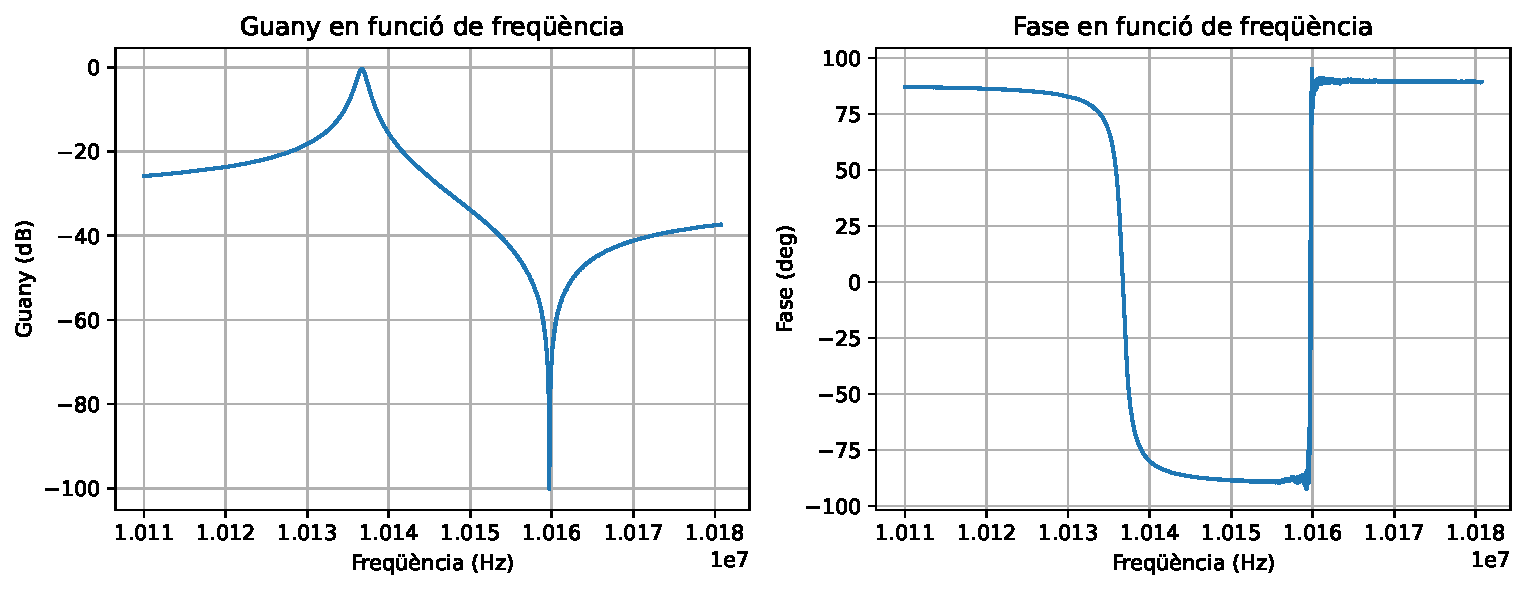
\includegraphics[width=\linewidth]{resposta_frequencial.pdf}
  \caption{Representació de la resposta freqüencial del circuit de mesura}
  \label{fig:resposta_frequencial}
\end{figure*}

\newthought{Pas 7:} Busquem a les mesures els valors de $f_0$, $f_{c1}$, $f_{c2}$ i $|H_{max}|$. Després aïllem de les expressions previament deduïdes.

\begin{table}
  \begin{center}
    \begin{tabular}{@{}rcccc@{}}
      \toprule
      Paràmetre & $R_m$ & $L_m$ & $C_m$ & $Q$ \\
      \midrule
      Expressió aïllada& $\frac{R_o}{|H_{max}|} - R_o$ & $\frac{R_m + R_o}{2 \pi BW}$ & $\frac{1}{L_m (2 \pi f_0)^2}$ & $\frac{f_0}{BW}$ \\
      \bottomrule
    \end{tabular}
  \end{center}
  \caption{Valors dels components en funció de les mesures i factor de qualitat}
\end{table}

\newthought{} Carreguem les dades per cercar els valors desitjats. La eïna escollida per dur a terme la operació ha estat Python.

\begin{minted}[
  frame=lines,
  framesep=2mm,
  baselinestretch=1.2,
  bgcolor=LightGray,
  fontsize=\footnotesize,
  linenos,
  breaklines
  ]{python}
  hmax_idx = modules.argmax()
  hmax = modules[hmax_idx]
  Ro = 50
  Rm = Ro/hmax - Ro
  fo = freqs[hmax_idx]
  fc1 = freqs[(np.abs(modules[:hmax_idx] - hmax/np.sqrt(2))).argmin()]
  fc2 = freqs[(np.abs(modules[hmax_idx:] - hmax/np.sqrt(2))).argmin() + hmax_idx]
  BW = fc2 - fc1
  Lm = (Ro + Rm)/(2 * pi * BW)
  Cm = 1/( (2 * pi * fo)**2 * Lm )
  Q = fo/BW
\end{minted}

\newthought{} En fer \mintinline{python}|print| dels valors obtenim les següents dades.\sidenote{Els calculs estàn fets amb unitats del sistema internacional}

\begin{minted}[
  frame=lines,
  framesep=2mm,
  baselinestretch=1.2,
  bgcolor=LightGray,
  fontsize=\footnotesize,
  linenos,
  breaklines
  ]{python}
  Rm = 2.309326308199182
  BW = 1330.0
  Lm = 0.006259614926132951
  Cm = 3.938223103179858e-14
  Q = 7621.571428571428
\end{minted}

\newthought{} Per obtenir $BW_u$ i $Q_u$ plantejem nodes al circuit de la figura \ref{fig:ideal_equiv} i normalitzem $H(s)$.

\begin{marginfigure}
  \begin{center}
    \begin{circuitikz}[transform shape, scale=0.9, baseline]
      \draw (0,0)node[below]{$+$} to[short, o-] ++(0.25,0) to[L=$L_m$] ++(1.5,0) to[C=$C_m$] ++(1.5,0) to[short, -*] ++(0.25,0) to[short, -o] ++(1.5,0)node[below]{$+$};
      \draw (3.5,0) to[R=$R_m$] ++(0,-2);
      \draw (0,-2)node[above]{$-$} to[short, o-*] ++(3.5,0) to[short, -o] ++(1.5,0)node[above]{$-$};
      \draw (-0.5,0) to[open=$v_{in}(t)$] ++(0,-2);
      \draw (4.5,0) to[open=$v_o(t)$] ++(0,-2);
    \end{circuitikz}
  \end{center}
  \caption{Circuit equivalent del cristall conectat a una font ideal}
  \label{fig:ideal_equiv}
\end{marginfigure}

\begin{gather*}
  V_o \left [ \frac{1}{R_m} + \frac{1}{L_m s + \frac{1}{C_m s}} \right ] = V_{in} \left [ \frac{1}{L_m s + \frac{1}{C_m s}} \right ]
  \\
  H(s) = \frac{\frac{1}{L_m s + \frac{1}{C_m s}}}{\frac{1}{R_m} + \frac{1}{L_m s + \frac{1}{C_m s}}}
  \\
  H(s) = \frac{R_m}{L_m} \cdot \frac{s}{s^2 + \frac{R_m}{L_m} s + \frac{1}{C_m L_m}}
\end{gather*}

\newthought{} D'aquesta manera es pot veure que $BW_u = \frac{R_m}{L_m}$ i que $Q_u = \frac{\omega_0}{BW_u} = \frac{1}{BW_u \sqrt{L_m C_m}}$. Ho calculem i queda.

\begin{minted}[
  frame=lines,
  framesep=2mm,
  baselinestretch=1.2,
  bgcolor=LightGray,
  fontsize=\footnotesize,
  linenos,
  breaklines
  ]{python}
  BWu = Rm/Lm
  Qu = 1/(BWu * np.sqrt(Lm * Cm))
\end{minted}

\begin{minted}[
  frame=lines,
  framesep=2mm,
  baselinestretch=1.2,
  bgcolor=LightGray,
  fontsize=\footnotesize,
  linenos,
  breaklines
  ]{python}
  BWu = 368.9246599751835
  Qu = 172638.7758295109
\end{minted}

\section{Determinació de $C_e$}

\newthought{Pas 8:} La freqüència $f_1$ a la qual es produeix la segona ressonància està situada al segón pic (el negatiu) de la gràfica de la figura \ref{fig:resposta_frequencial}. És una frequencia de ressonància perque la fase és nula, i és negativa perque la impedància del cristall és molt alta. Tal i com s'ha raonat anteriorment.

\newthought{} El valor de $f_1$ rondarà els \qty{10.16}{\mega\hertz}.

\newthought{} Per coneixer el valor de la impedància i la admitància amb exactitud executem les següents línies de codi.

\begin{minted}[
  frame=lines,
  framesep=2mm,
  baselinestretch=1.2,
  bgcolor=LightGray,
  fontsize=\footnotesize,
  linenos,
  breaklines
  ]{python}
  f1 = freqs[modules.argmin()]
  Zs = Rm + 1j*(Lm * f1 * 2*pi - 1/(Cm * f1 * 2*pi))
  Ys = 1/Zs
  Rp = 1/(Ys.real)
  Lp = -1/(Ys.imag * f1 * 2*pi)
\end{minted}

\begin{minted}[
  frame=lines,
  framesep=2mm,
  baselinestretch=1.2,
  bgcolor=LightGray,
  fontsize=\footnotesize,
  linenos,
  breaklines
  ]{python}
  f1 = 10159700.0
  Zs = (2.309326308199182+1807.9317002811003j)
  Ys = (7.065136469458759e-07-0.0005531173374934277j)
  Rp = 1415400.8267537504
  Lp = 2.8321873317442023e-05
\end{minted}

\newthought{} Aquesta admitància ens indica que el conjunt pot ser expressat com es mostra a la figura \ref{fig:high_freq_equiv}, on $L_p \simeq \qty{28.32}{\micro\henry}$ i $R_p \simeq \qty{1.41}{\mega\ohm}$.

\newthought{} Com per $f_1$ hi ha ressonància, sabem que en aquesta configuració la admitància del inductor $L_p$ i el condensador $C_e$ han de sumar $0$.

\begin{gather*}
  \Im (Y_s) + C_e(2\pi f_1) = 0 \\
  C_e = \frac{- \Im (Y_s)}{2\pi f_1}
\end{gather*}

\newthought{} En codi

\begin{minted}[
  frame=lines,
  framesep=2mm,
  baselinestretch=1.2,
  bgcolor=LightGray,
  fontsize=\footnotesize,
  linenos,
  breaklines
  ]{python}
  Ce = -(Ys.imag)/(2*pi * f1)
\end{minted}

\begin{minted}[
  frame=lines,
  framesep=2mm,
  baselinestretch=1.2,
  bgcolor=LightGray,
  fontsize=\footnotesize,
  linenos,
  breaklines
  ]{python}
  Ce = 8.66475962596407e-12
\end{minted}

\newthought{} La taula \ref{table:all_values} és la recopilació de totes les dades obtingudes.

\begin{table}
  \begin{center}
    \begin{tabular}{@{}cc|cc@{}}
      \toprule
      Paràmetre & Valor mesurat & Element & Valor calculat \\      
      \midrule
      $|H_{max}|$ & \num{0.9558} & $R_m$ & \qty{2.309}{\ohm} \\
      $BW$ & \qty{1330}{\hertz} & $L_m$ & \qty{6.259}{\milli\henry} \\
      $f_0$ & \qty{10.136}{\mega\hertz} & $C_m$ & \qty{0.03938}{\pico\farad} \\
      $f_1$ & \qty{10.160}{\mega\hertz} & $C_e$ & \qty{8.664}{\pico\farad} \\
      \bottomrule
      Paràmetre & Valor calculat & & \\
      \midrule
      $Q$ & \num{7621} && \\
      $Q_u$ & \num{172638} && \\
      \bottomrule
    \end{tabular}
  \end{center}
  \caption{Deducció dels valors del model del cristall}
  \label{table:all_values}
\end{table}

\section{Validació de resultats}

\newthought{Pas 9:} El resultat es troba a la figura \ref{fig:comparation}. Es pot apreciar un cert desfasament entre les respostes. Això és degut en major part a imprecisió a l'hora de entrar els valors dels components al simulador. Tret d'aquest detall el model funciona practicament igual entre les freqüencies desitjades que el quars.

\begin{figure}
  \begin{center}
    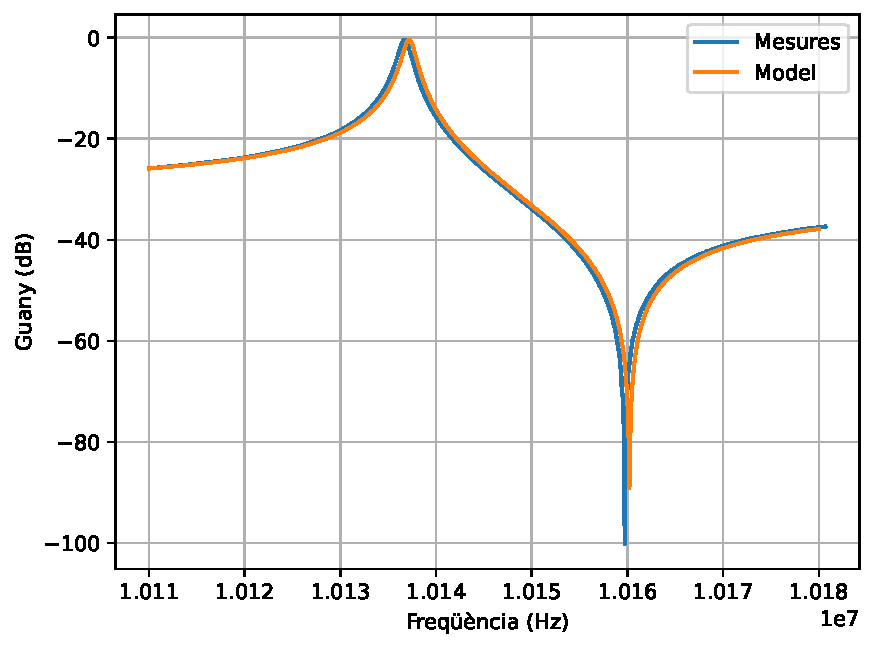
\includegraphics[width=\linewidth]{comparacio.pdf}
  \end{center}
  \caption{Dades simulades sobre dades mesurades}
  \label{fig:comparation}
\end{figure}

\section{Aplicació al filtrat de senyals}

\newthought{Pas 10:} Normalment s'hauria de calcular les integrals corresponents per obtenir els coeficients de Fourier, de tota manera també podem observar el següent.\sidenote{El raonament fa us de la famosa formula $\cos^2(x) = \frac{1 + cos(2x)}{2}$}

\begin{align*}
  v_g(t) &= 6 \cdot \cos^2(2\pi f_x t) \\
  &= 6 \left ( \frac{1 + \cos \left ( 2 (2\pi f_x t) \right )}{2} \right ) \\
  &= 3 + 3\cos(4\pi f_x t)
\end{align*}

\newthought{} Aquesta última expressió ja és una combinació lineal de cosinus. Per tant, equival al seu desenvolupament de Fourier.

\newthought{Pas 11:} Per $f_x = \frac{f_o}{2}$, $v_g(t) = 3+3\cos(2\pi f_o t)$. La component continua serà gairebé completament eliminada pel filtre, d'altra banda, el cosinus no serà gaire atenuat i gens desfasat.\sidenote[][-27px]{Com la freqüència del cosinus és la de ressonància la fase que aporta el filtre es nula. La atenuació es notable pero baixa.}

\begin{figure*}
  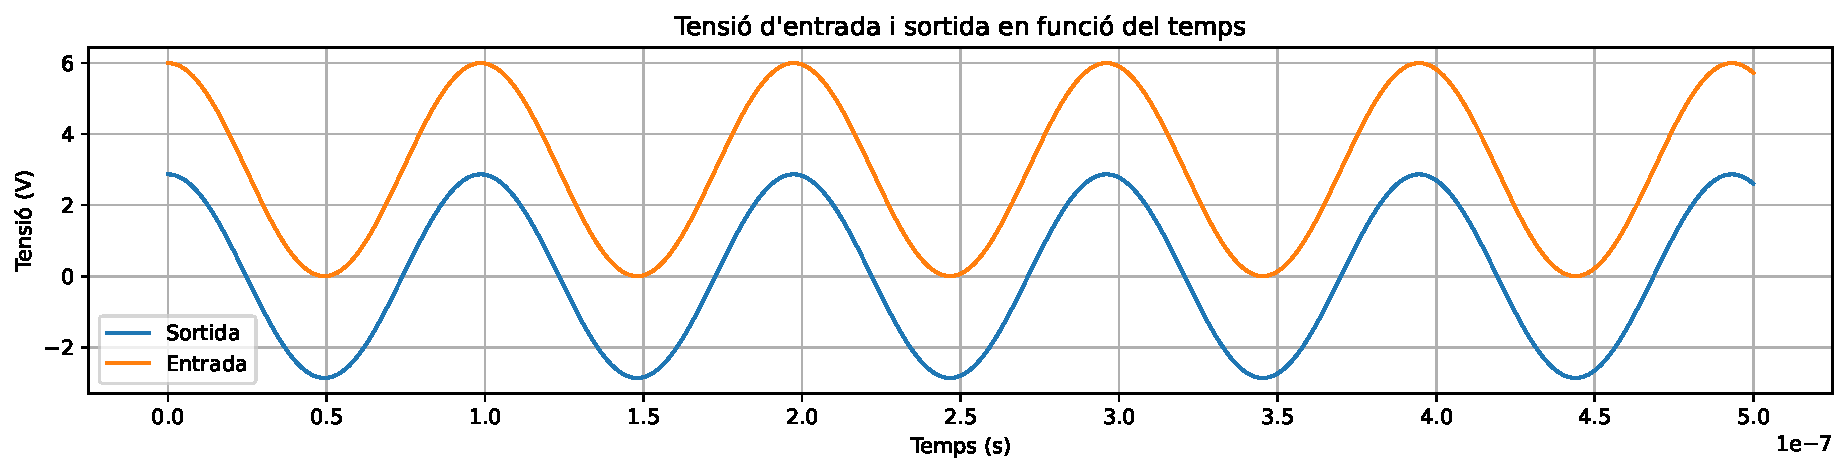
\includegraphics[width=\linewidth]{sortida1.pdf}
  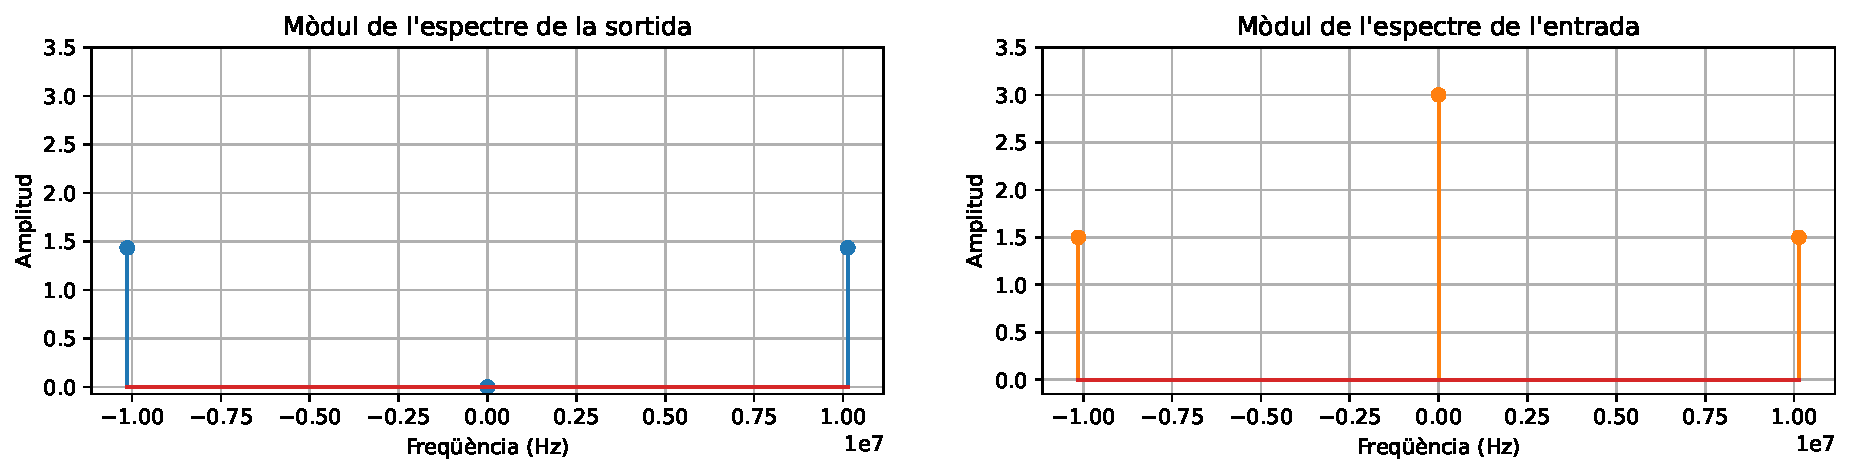
\includegraphics[width=\linewidth]{sortida2.pdf}
  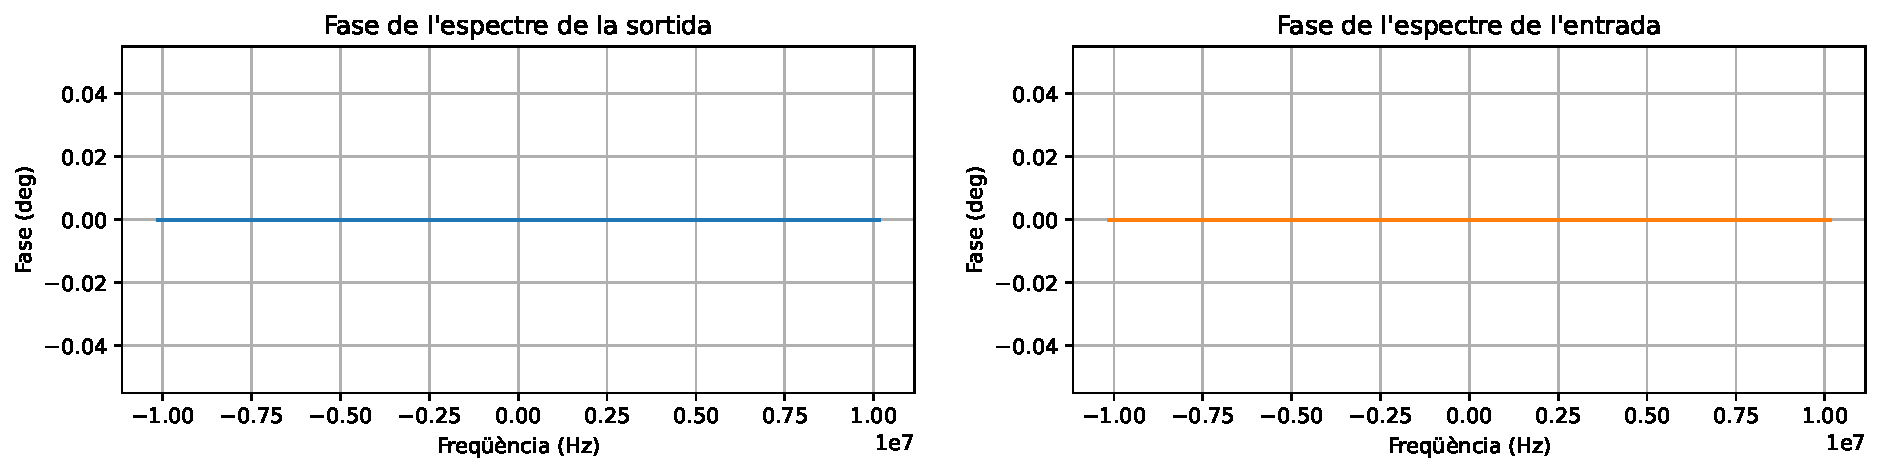
\includegraphics[width=\linewidth]{sortida3.pdf}
  \caption{Anàlisi de l'entrada $v_g$ i la sortida del filtre}
\end{figure*}

\end{document}